
Com o intuito de planejar a Verificação e Validação da Interface Gráfica que compõe o sistema Enturma, primeiramente precisamos compreender as funcionalidades principais do sistema, seu objetivo principal, seus objetivos secundários e os pontos mais críticos do sistema.

O sistema Enturma possui como objetivo, informar a população brasileira sobre o desempenho das turmas escolares no país, facilitando o conhecimento a cerca da distribuição de ensino por todo o país, apresentando com clareza as diferenças entre cada estado e seus tipos escolares (público, privado, estadual, municipal). 

Obter a informação a cerca de uma determinada turma é o principal objetivo do sistema, já que o usuário poderá saber a evolução de sua turma, podendo compará-la com outras turmas, de outros estados por exemplo. O \textit{framework do problema} pode ser observado na tabela \ref{tab:problema}.


\begin{table}[H]
	\centering
	\begin{tabular}{|l|l|}
		\hline
		\textbf{O problema de}                    & \begin{tabular}[c]{@{}l@{}}Falta de conhecimento a cerca do desempenho\\ das turmas escolares brasileiras.\end{tabular}                                                                                                                                                                         \\ \hline
		\textbf{Afeta}                            & Todos os brasileiros.                                                                                                                                                                                                                                                                           \\ \hline
		\textbf{Cujo impacto é}                   & \begin{tabular}[c]{@{}l@{}}O decaimento do rendimento dos alunos fica a margem \\ do conhecimento da população brasileira, estando essa \\ sem ter como acompanhar quando é que a educação \\ começa a oscilar para poder exigir investimento de \\ recursos por parte do governo.\end{tabular} \\ \hline
		\textbf{Benefícios de uma solução seriam} & \begin{tabular}[c]{@{}l@{}}Exigência por parte da população para a elaboração de \\ leis e medidas que focariam melhorias na educação em \\ fases críticas do ensino, as quais se apresentam \\ defasadas nos resultados das provas avaliativas.\end{tabular}                                   \\ \hline
	\end{tabular}
	\caption{Framework de Problema}
	\label{tab:problema}
\end{table}

\subsection{Recursos do produto} % (fold)
\label{sub:recursos_do_produto}


Os usuários finais do sistema EnTurma possuem como maior necessidade a de visualizar o desempenho de uma determinada turma do sistema educacional brasileiro. A tabela \ref{tab:recursos} apresenta todos os recursos do sistema e suas características.

\begin{table}[H]
	\centering
	\begin{tabular}{|l|l|}
		\hline
		\textbf{Necessidade}      & \textbf{Características}                                                                                                                                                                                                                                                                                                   \\ \hline
		Gerar relatório da turma  & \begin{tabular}[c]{@{}l@{}}Os gráficos podem ser gerados a partir dos indicadores \\ e período escolhidos. Os indicadores podem ser: média\\  dos alunos, média de horas/aula, taxa de rendimento, \\ e outros. O período escolhido pode variar entre 2006 a \\ 2014 dependendo da disponibilidade dos dados.\end{tabular} \\ \hline
		Comparar turmas           & \begin{tabular}[c]{@{}l@{}}Comparação de duas turmas em um mesmo indicador. \\ Exemplo: comparar a turma da primeira série do ano \\ de 2007 com a de 2008 em relação à média escolar.\end{tabular}                                                                                                                        \\ \hline
		Gerar ranking             & \begin{tabular}[c]{@{}l@{}}O sistema deve gerar ranking dos melhores estados em \\ um determinado indicador.\end{tabular}                                                                                                                                                                                                  \\ \hline
		Contactar desenvolvedores & \begin{tabular}[c]{@{}l@{}}O sistema disponibiliza uma seção que permite que o \\ usuário entre em contato com os desenvolvedores a fim \\ de sanar dúvidas, fazer críticas ou sugestões sobre o sistema.\end{tabular}                                                                                                     \\ \hline
	\end{tabular}
	\caption{Recursos do Sistema}
	\label{tab:recursos}
\end{table}

	O relacionamento destes recursos com os Atores do sistema pode ser observado na Modelagem de Casos de Uso do Sistema Enturma, que está disposta na figura \ref{img:modelagem}.

	\begin{figure}[H]
		\centering
		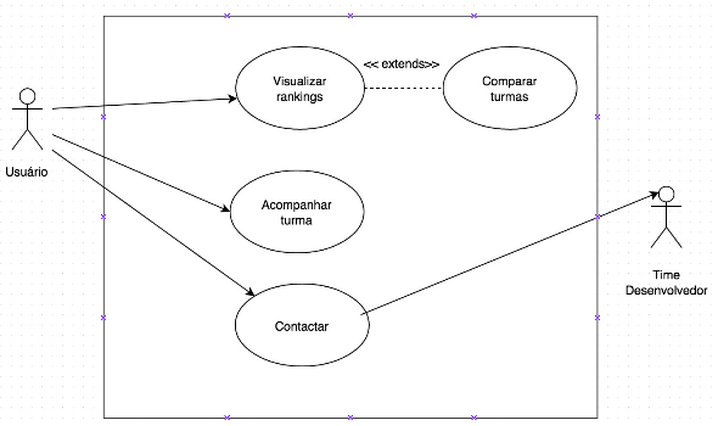
\includegraphics[width=0.7\textwidth]{imagens/modelagem}
		\caption{Modelagem de Casos de Uso}
		\label{img:modelagem}
	\end{figure}



% subsection recursos_do_produto (end)